\section{Quantum Modulation}
    As in a classical system, it is possible to define the concept of modulation for a 
    quantum communication system. The trasmitted information, will be associated to a 
    quantum state of the electromagnetic field, so it can be trasmitted on the communication 
    channel.

    \begin{figure}[ht]
        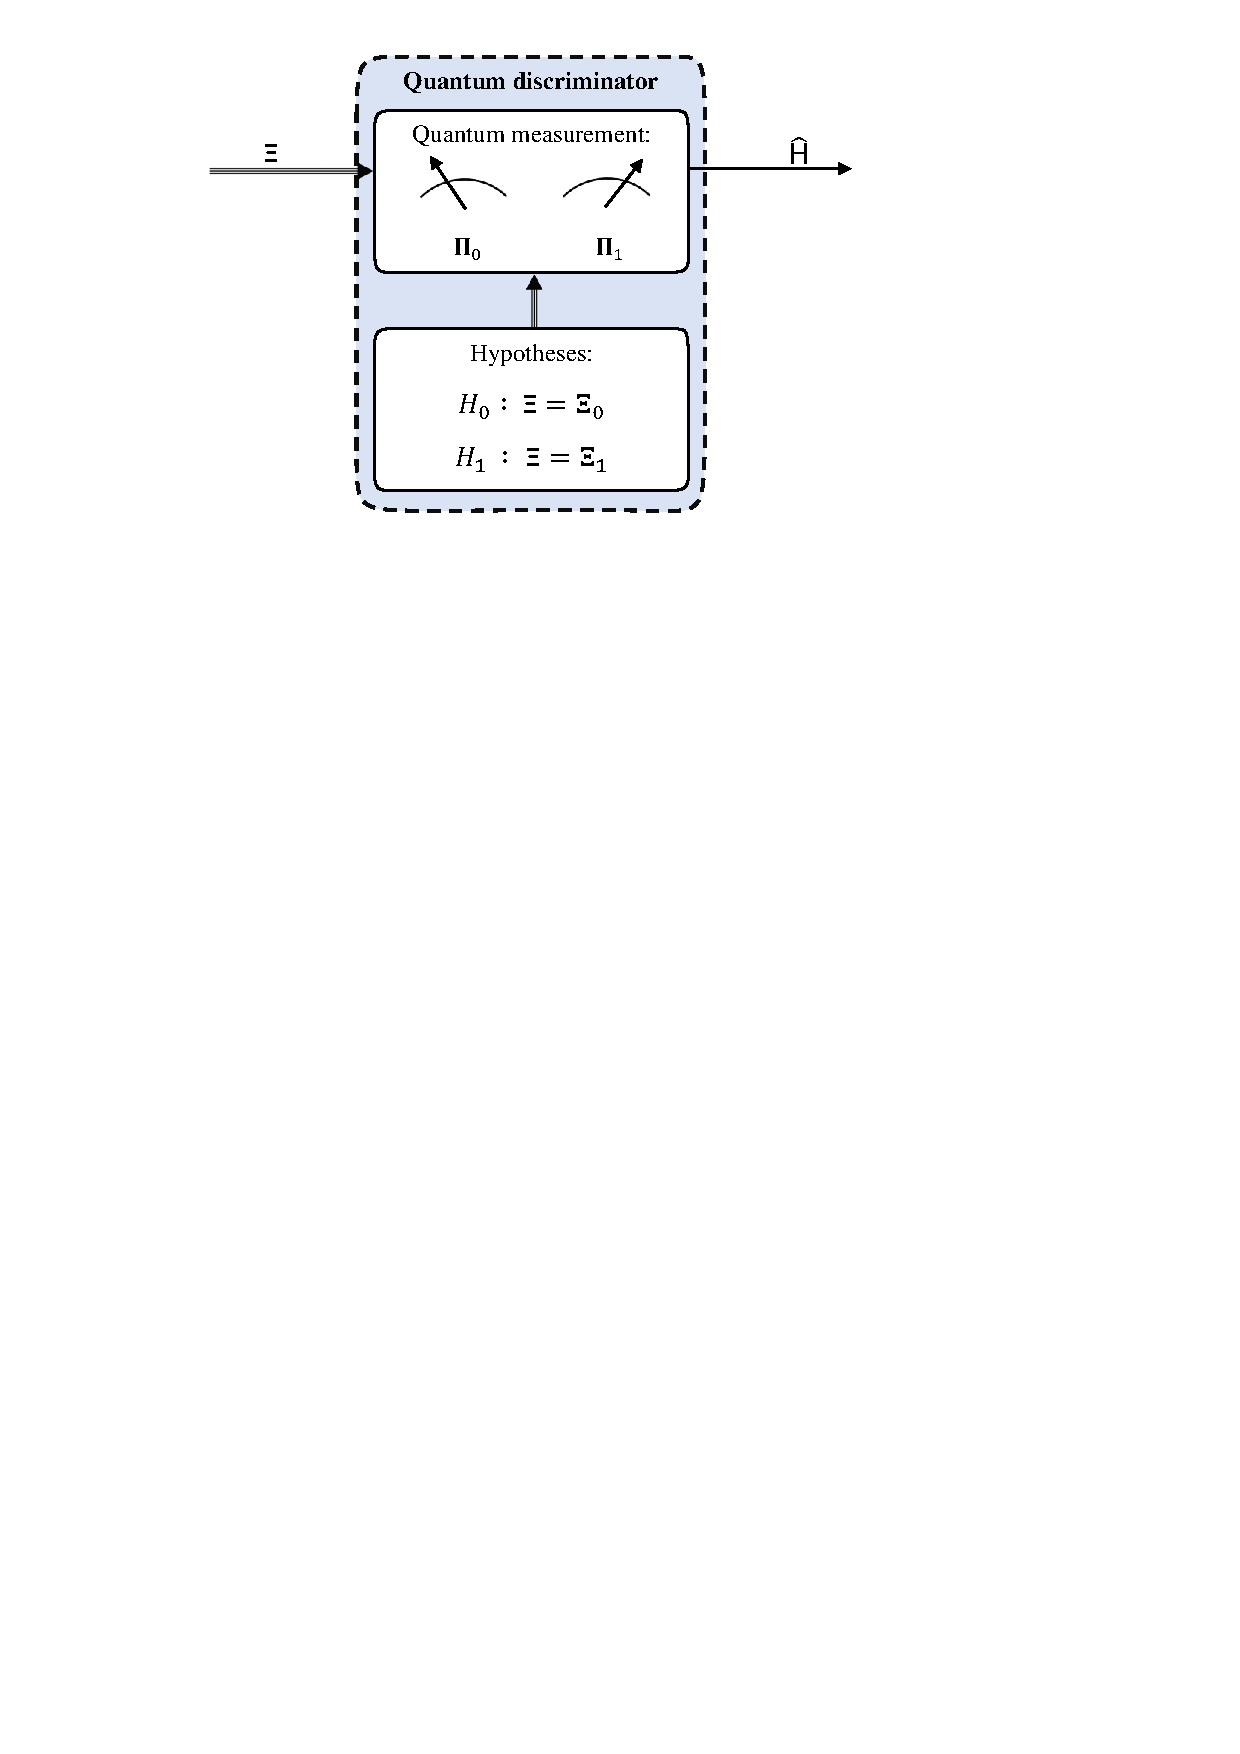
\includegraphics[width=1\textwidth]{fig2.1.pdf}
        \caption{Block diagram of a quantum trasmitter.}
        \label{fig:2.1}
    \end{figure}
    It is possible to think about the quantum trasmitter as in figure \ref{fig:2.1}. The bit source
    emits a bit sequence, the serial-parallel converter parallelize a group of $l$-bit (where, if $L$
    is the number of quantum states, $l=\log_2(L)$) and sends them to the quantum modulator; this last
    associate to every group of bit, one quantum state. The operation of quantum state creation, 
    in real cases, is affected by noise.

    The sequence of operation is very closer to a classical trasmitter, the main difference is that
    the modulator map the bits into quantum states instead of classical modulation. It is, therefor, 
    possible to achieve the equivalent of classical modulation, that it is called quantum modulation,
    with several states and assess the impact on performance.
    In this thesis only the binary will be considered and assessed, in the OOK and BPSK configuration.
    
    \subsection{OOK modulation}

    \subsection{BPSK modulation}
